% Figure 1: Venn diagram of three lineages — standalone file
% Drop into the paper with % Figure 1: Venn diagram of three lineages — standalone file
% Drop into the paper with % Figure 1: Venn diagram of three lineages — standalone file
% Drop into the paper with % Figure 1: Venn diagram of three lineages — standalone file
% Drop into the paper with \input{figure_venn}
%
% Requires: tikz, xcolor
% Compile:  pdflatex figure_venn.tex

\documentclass[tikz,11pt]{standalone}
\usepackage{xcolor}
\usepackage{tikz}
\usetikzlibrary{arrows.meta, positioning, calc, shadows}

\definecolor{okblue}{HTML}{0072B2}
\definecolor{okorange}{HTML}{E69F00}
\definecolor{okgreen}{HTML}{009E73}
\definecolor{okred}{HTML}{D55E00}
\definecolor{okyellow}{HTML}{F0E442}
\definecolor{okgray}{HTML}{999999}

\begin{document}
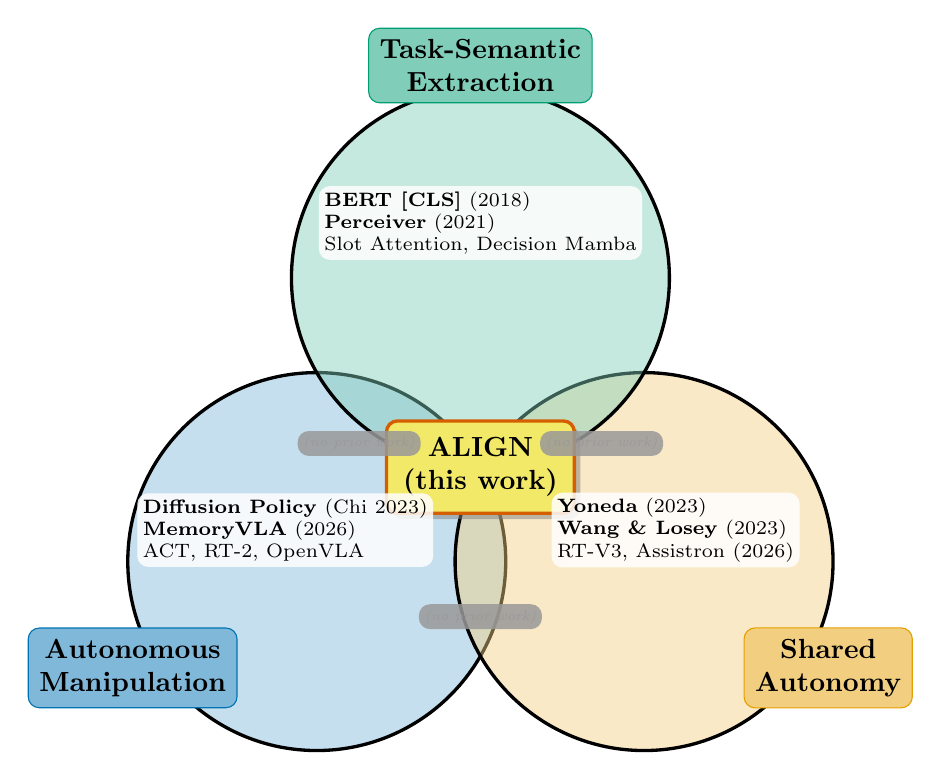
\begin{tikzpicture}[
    every node/.style={font=\small},
    circ/.style={draw, very thick, fill opacity=0.45, text opacity=1,
                 line width=1.2pt},
]
\def\R{2.4}
\def\RC{2.4}

\coordinate (figC)   at (0, 0);
\coordinate (cA)     at (210:\RC);
\coordinate (cB)     at (330:\RC);
\coordinate (cC)     at (90:\RC);

\draw[circ, fill=okblue!50]   (cA) circle (\R);
\draw[circ, fill=okorange!50] (cB) circle (\R);
\draw[circ, fill=okgreen!50]  (cC) circle (\R);

\node[font=\bfseries, fill=okblue!50, draw=okblue, rounded corners,
      inner sep=4pt, align=center]
    at ($(cA)+(210:2.7)$) {Autonomous\\Manipulation};
\node[font=\bfseries, fill=okorange!50, draw=okorange, rounded corners,
      inner sep=4pt, align=center]
    at ($(cB)+(330:2.7)$) {Shared\\Autonomy};
\node[font=\bfseries, fill=okgreen!50, draw=okgreen, rounded corners,
      inner sep=4pt, align=center]
    at ($(cC)+(90:2.7)$) {Task-Semantic\\Extraction};

\node[draw=okred, very thick, fill=okyellow!80, rounded corners,
      inner sep=6pt, align=center, font=\bfseries, drop shadow]
    at (figC) {ALIGN\\(this work)};

\node[align=left, font=\scriptsize, fill=white, fill opacity=0.85, text opacity=1,
      inner sep=2pt, rounded corners]
    at ($(cA)+(-0.4, 0.4)$)
    {\textbf{Diffusion Policy} (Chi 2023)\\
     \textbf{MemoryVLA} (2026)\\
     ACT, RT-2, OpenVLA};
\node[align=left, font=\scriptsize, fill=white, fill opacity=0.85, text opacity=1,
      inner sep=2pt, rounded corners]
    at ($(cB)+(0.4, 0.4)$)
    {\textbf{Yoneda} (2023)\\
     \textbf{Wang \& Losey} (2023)\\
     RT-V3, Assistron (2026)};
\node[align=left, font=\scriptsize, fill=white, fill opacity=0.85, text opacity=1,
      inner sep=2pt, rounded corners]
    at ($(cC)+(0, 0.7)$)
    {\textbf{BERT [CLS]} (2018)\\
     \textbf{Perceiver} (2021)\\
     Slot Attention, Decision Mamba};

\node[font=\tiny\itshape, fill=white, fill opacity=0.85, text opacity=1,
      inner sep=2pt, rounded corners, color=okgray, align=center]
    at ($(cA)!0.5!(cB)+(0,-0.7)$)
    {(no prior work)};
\node[font=\tiny\itshape, fill=white, fill opacity=0.85, text opacity=1,
      inner sep=2pt, rounded corners, color=okgray]
    at ($(cA)!0.5!(cC)+(-0.5,-0.3)$) {(no prior work)};
\node[font=\tiny\itshape, fill=white, fill opacity=0.85, text opacity=1,
      inner sep=2pt, rounded corners, color=okgray]
    at ($(cB)!0.5!(cC)+(0.5,-0.3)$) {(no prior work)};
\end{tikzpicture}
\end{document}

%
% Requires: tikz, xcolor
% Compile:  pdflatex figure_venn.tex

\documentclass[tikz,11pt]{standalone}
\usepackage{xcolor}
\usepackage{tikz}
\usetikzlibrary{arrows.meta, positioning, calc, shadows}

\definecolor{okblue}{HTML}{0072B2}
\definecolor{okorange}{HTML}{E69F00}
\definecolor{okgreen}{HTML}{009E73}
\definecolor{okred}{HTML}{D55E00}
\definecolor{okyellow}{HTML}{F0E442}
\definecolor{okgray}{HTML}{999999}

\begin{document}
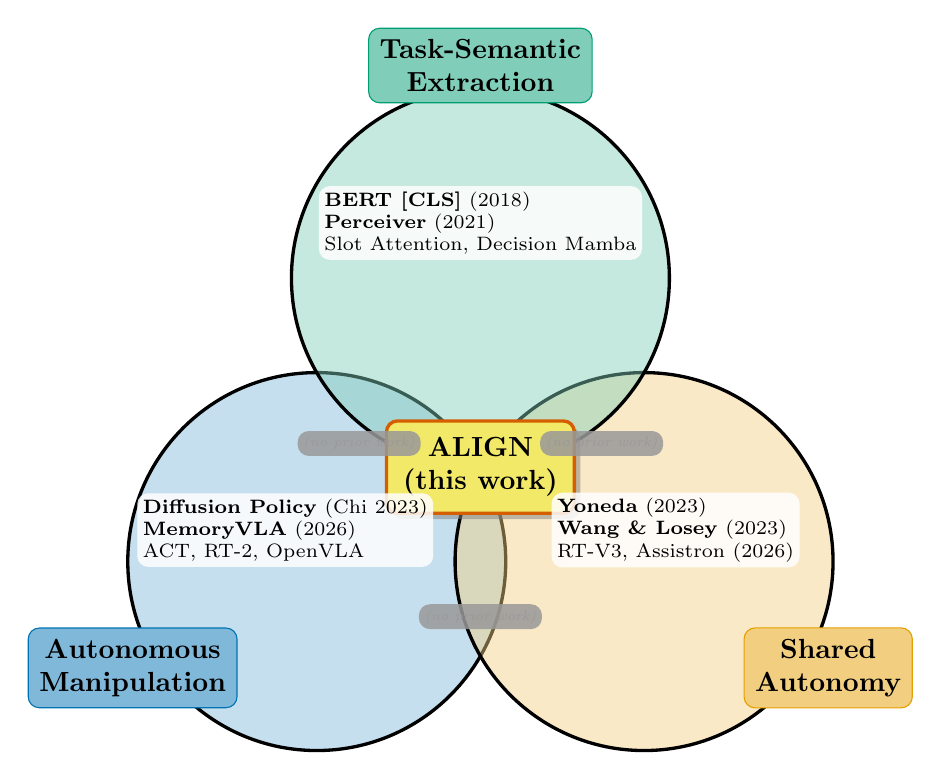
\begin{tikzpicture}[
    every node/.style={font=\small},
    circ/.style={draw, very thick, fill opacity=0.45, text opacity=1,
                 line width=1.2pt},
]
\def\R{2.4}
\def\RC{2.4}

\coordinate (figC)   at (0, 0);
\coordinate (cA)     at (210:\RC);
\coordinate (cB)     at (330:\RC);
\coordinate (cC)     at (90:\RC);

\draw[circ, fill=okblue!50]   (cA) circle (\R);
\draw[circ, fill=okorange!50] (cB) circle (\R);
\draw[circ, fill=okgreen!50]  (cC) circle (\R);

\node[font=\bfseries, fill=okblue!50, draw=okblue, rounded corners,
      inner sep=4pt, align=center]
    at ($(cA)+(210:2.7)$) {Autonomous\\Manipulation};
\node[font=\bfseries, fill=okorange!50, draw=okorange, rounded corners,
      inner sep=4pt, align=center]
    at ($(cB)+(330:2.7)$) {Shared\\Autonomy};
\node[font=\bfseries, fill=okgreen!50, draw=okgreen, rounded corners,
      inner sep=4pt, align=center]
    at ($(cC)+(90:2.7)$) {Task-Semantic\\Extraction};

\node[draw=okred, very thick, fill=okyellow!80, rounded corners,
      inner sep=6pt, align=center, font=\bfseries, drop shadow]
    at (figC) {ALIGN\\(this work)};

\node[align=left, font=\scriptsize, fill=white, fill opacity=0.85, text opacity=1,
      inner sep=2pt, rounded corners]
    at ($(cA)+(-0.4, 0.4)$)
    {\textbf{Diffusion Policy} (Chi 2023)\\
     \textbf{MemoryVLA} (2026)\\
     ACT, RT-2, OpenVLA};
\node[align=left, font=\scriptsize, fill=white, fill opacity=0.85, text opacity=1,
      inner sep=2pt, rounded corners]
    at ($(cB)+(0.4, 0.4)$)
    {\textbf{Yoneda} (2023)\\
     \textbf{Wang \& Losey} (2023)\\
     RT-V3, Assistron (2026)};
\node[align=left, font=\scriptsize, fill=white, fill opacity=0.85, text opacity=1,
      inner sep=2pt, rounded corners]
    at ($(cC)+(0, 0.7)$)
    {\textbf{BERT [CLS]} (2018)\\
     \textbf{Perceiver} (2021)\\
     Slot Attention, Decision Mamba};

\node[font=\tiny\itshape, fill=white, fill opacity=0.85, text opacity=1,
      inner sep=2pt, rounded corners, color=okgray, align=center]
    at ($(cA)!0.5!(cB)+(0,-0.7)$)
    {(no prior work)};
\node[font=\tiny\itshape, fill=white, fill opacity=0.85, text opacity=1,
      inner sep=2pt, rounded corners, color=okgray]
    at ($(cA)!0.5!(cC)+(-0.5,-0.3)$) {(no prior work)};
\node[font=\tiny\itshape, fill=white, fill opacity=0.85, text opacity=1,
      inner sep=2pt, rounded corners, color=okgray]
    at ($(cB)!0.5!(cC)+(0.5,-0.3)$) {(no prior work)};
\end{tikzpicture}
\end{document}

%
% Requires: tikz, xcolor
% Compile:  pdflatex figure_venn.tex

\documentclass[tikz,11pt]{standalone}
\usepackage{xcolor}
\usepackage{tikz}
\usetikzlibrary{arrows.meta, positioning, calc, shadows}

\definecolor{okblue}{HTML}{0072B2}
\definecolor{okorange}{HTML}{E69F00}
\definecolor{okgreen}{HTML}{009E73}
\definecolor{okred}{HTML}{D55E00}
\definecolor{okyellow}{HTML}{F0E442}
\definecolor{okgray}{HTML}{999999}

\begin{document}
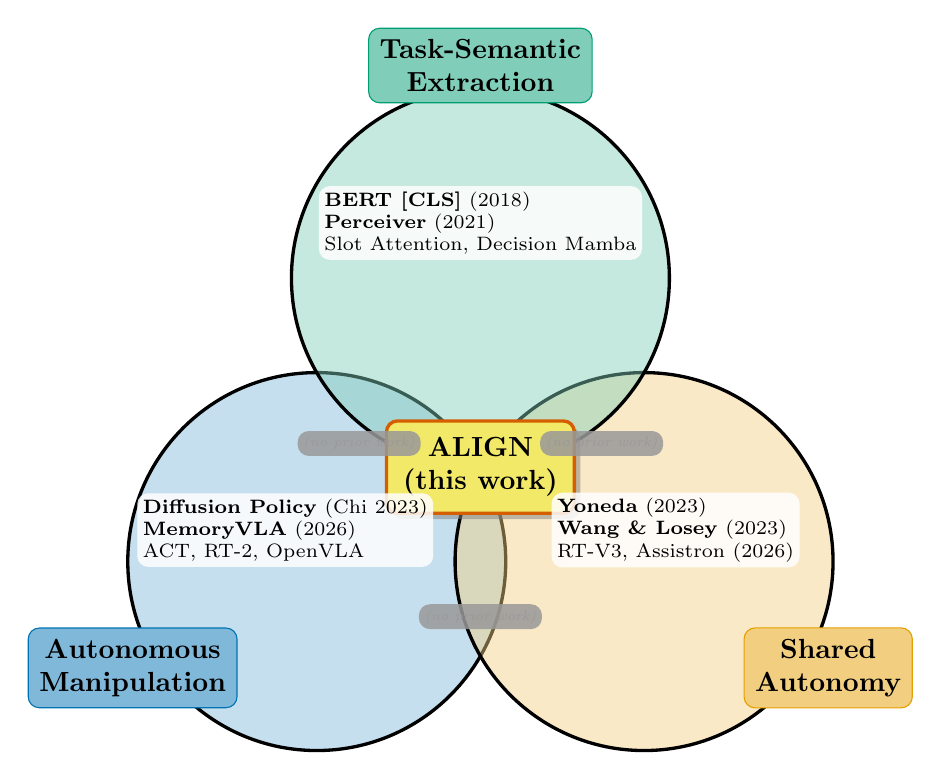
\begin{tikzpicture}[
    every node/.style={font=\small},
    circ/.style={draw, very thick, fill opacity=0.45, text opacity=1,
                 line width=1.2pt},
]
\def\R{2.4}
\def\RC{2.4}

\coordinate (figC)   at (0, 0);
\coordinate (cA)     at (210:\RC);
\coordinate (cB)     at (330:\RC);
\coordinate (cC)     at (90:\RC);

\draw[circ, fill=okblue!50]   (cA) circle (\R);
\draw[circ, fill=okorange!50] (cB) circle (\R);
\draw[circ, fill=okgreen!50]  (cC) circle (\R);

\node[font=\bfseries, fill=okblue!50, draw=okblue, rounded corners,
      inner sep=4pt, align=center]
    at ($(cA)+(210:2.7)$) {Autonomous\\Manipulation};
\node[font=\bfseries, fill=okorange!50, draw=okorange, rounded corners,
      inner sep=4pt, align=center]
    at ($(cB)+(330:2.7)$) {Shared\\Autonomy};
\node[font=\bfseries, fill=okgreen!50, draw=okgreen, rounded corners,
      inner sep=4pt, align=center]
    at ($(cC)+(90:2.7)$) {Task-Semantic\\Extraction};

\node[draw=okred, very thick, fill=okyellow!80, rounded corners,
      inner sep=6pt, align=center, font=\bfseries, drop shadow]
    at (figC) {ALIGN\\(this work)};

\node[align=left, font=\scriptsize, fill=white, fill opacity=0.85, text opacity=1,
      inner sep=2pt, rounded corners]
    at ($(cA)+(-0.4, 0.4)$)
    {\textbf{Diffusion Policy} (Chi 2023)\\
     \textbf{MemoryVLA} (2026)\\
     ACT, RT-2, OpenVLA};
\node[align=left, font=\scriptsize, fill=white, fill opacity=0.85, text opacity=1,
      inner sep=2pt, rounded corners]
    at ($(cB)+(0.4, 0.4)$)
    {\textbf{Yoneda} (2023)\\
     \textbf{Wang \& Losey} (2023)\\
     RT-V3, Assistron (2026)};
\node[align=left, font=\scriptsize, fill=white, fill opacity=0.85, text opacity=1,
      inner sep=2pt, rounded corners]
    at ($(cC)+(0, 0.7)$)
    {\textbf{BERT [CLS]} (2018)\\
     \textbf{Perceiver} (2021)\\
     Slot Attention, Decision Mamba};

\node[font=\tiny\itshape, fill=white, fill opacity=0.85, text opacity=1,
      inner sep=2pt, rounded corners, color=okgray, align=center]
    at ($(cA)!0.5!(cB)+(0,-0.7)$)
    {(no prior work)};
\node[font=\tiny\itshape, fill=white, fill opacity=0.85, text opacity=1,
      inner sep=2pt, rounded corners, color=okgray]
    at ($(cA)!0.5!(cC)+(-0.5,-0.3)$) {(no prior work)};
\node[font=\tiny\itshape, fill=white, fill opacity=0.85, text opacity=1,
      inner sep=2pt, rounded corners, color=okgray]
    at ($(cB)!0.5!(cC)+(0.5,-0.3)$) {(no prior work)};
\end{tikzpicture}
\end{document}

%
% Requires: tikz, xcolor
% Compile:  pdflatex figure_venn.tex

\documentclass[tikz,11pt]{standalone}
\usepackage{xcolor}
\usepackage{tikz}
\usetikzlibrary{arrows.meta, positioning, calc, shadows}

\definecolor{okblue}{HTML}{0072B2}
\definecolor{okorange}{HTML}{E69F00}
\definecolor{okgreen}{HTML}{009E73}
\definecolor{okred}{HTML}{D55E00}
\definecolor{okyellow}{HTML}{F0E442}
\definecolor{okgray}{HTML}{999999}

\begin{document}
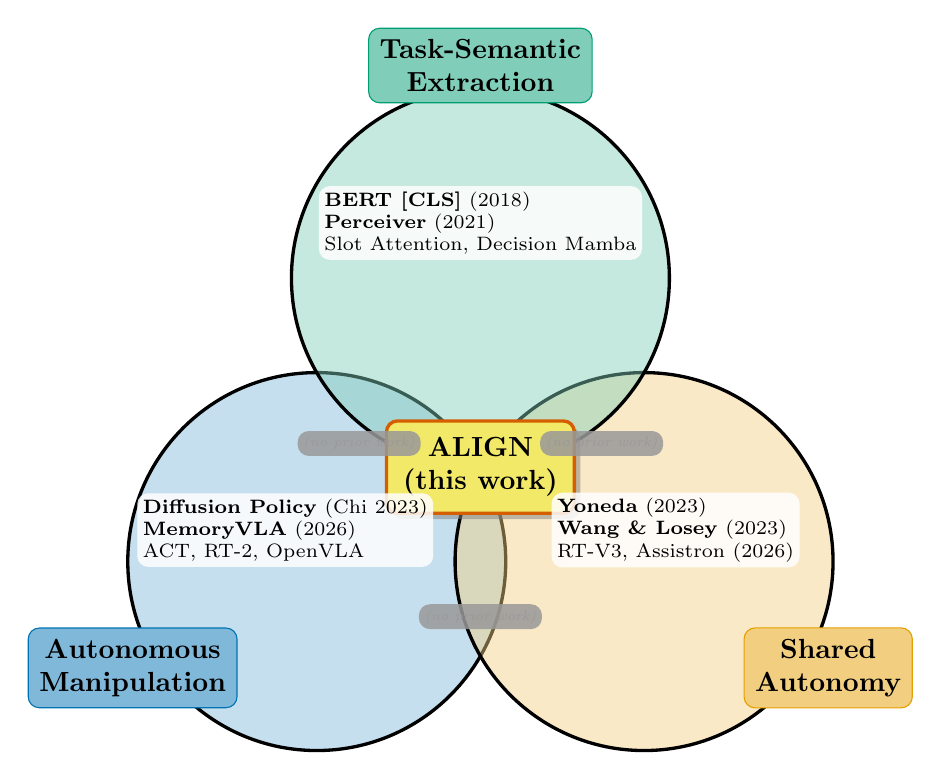
\begin{tikzpicture}[
    every node/.style={font=\small},
    circ/.style={draw, very thick, fill opacity=0.45, text opacity=1,
                 line width=1.2pt},
]
\def\R{2.4}
\def\RC{2.4}

\coordinate (figC)   at (0, 0);
\coordinate (cA)     at (210:\RC);
\coordinate (cB)     at (330:\RC);
\coordinate (cC)     at (90:\RC);

\draw[circ, fill=okblue!50]   (cA) circle (\R);
\draw[circ, fill=okorange!50] (cB) circle (\R);
\draw[circ, fill=okgreen!50]  (cC) circle (\R);

\node[font=\bfseries, fill=okblue!50, draw=okblue, rounded corners,
      inner sep=4pt, align=center]
    at ($(cA)+(210:2.7)$) {Autonomous\\Manipulation};
\node[font=\bfseries, fill=okorange!50, draw=okorange, rounded corners,
      inner sep=4pt, align=center]
    at ($(cB)+(330:2.7)$) {Shared\\Autonomy};
\node[font=\bfseries, fill=okgreen!50, draw=okgreen, rounded corners,
      inner sep=4pt, align=center]
    at ($(cC)+(90:2.7)$) {Task-Semantic\\Extraction};

\node[draw=okred, very thick, fill=okyellow!80, rounded corners,
      inner sep=6pt, align=center, font=\bfseries, drop shadow]
    at (figC) {ALIGN\\(this work)};

\node[align=left, font=\scriptsize, fill=white, fill opacity=0.85, text opacity=1,
      inner sep=2pt, rounded corners]
    at ($(cA)+(-0.4, 0.4)$)
    {\textbf{Diffusion Policy} (Chi 2023)\\
     \textbf{MemoryVLA} (2026)\\
     ACT, RT-2, OpenVLA};
\node[align=left, font=\scriptsize, fill=white, fill opacity=0.85, text opacity=1,
      inner sep=2pt, rounded corners]
    at ($(cB)+(0.4, 0.4)$)
    {\textbf{Yoneda} (2023)\\
     \textbf{Wang \& Losey} (2023)\\
     RT-V3, Assistron (2026)};
\node[align=left, font=\scriptsize, fill=white, fill opacity=0.85, text opacity=1,
      inner sep=2pt, rounded corners]
    at ($(cC)+(0, 0.7)$)
    {\textbf{BERT [CLS]} (2018)\\
     \textbf{Perceiver} (2021)\\
     Slot Attention, Decision Mamba};

\node[font=\tiny\itshape, fill=white, fill opacity=0.85, text opacity=1,
      inner sep=2pt, rounded corners, color=okgray, align=center]
    at ($(cA)!0.5!(cB)+(0,-0.7)$)
    {(no prior work)};
\node[font=\tiny\itshape, fill=white, fill opacity=0.85, text opacity=1,
      inner sep=2pt, rounded corners, color=okgray]
    at ($(cA)!0.5!(cC)+(-0.5,-0.3)$) {(no prior work)};
\node[font=\tiny\itshape, fill=white, fill opacity=0.85, text opacity=1,
      inner sep=2pt, rounded corners, color=okgray]
    at ($(cB)!0.5!(cC)+(0.5,-0.3)$) {(no prior work)};
\end{tikzpicture}
\end{document}
